\documentclass[12pt]{article} % Tamaño de fuente y tipo de documento
\usepackage[utf8]{inputenc}
%\usepackage{tikz} % Gráficos
\usepackage{amsmath} % Formulas matemáticas
\usepackage{setspace} % Espacio entre líneas
\usepackage{indentfirst} % Sangría en primeros párrafos de sección
\usepackage{lipsum} % Texto de prueba
\usepackage{fancyhdr} % Personalizar estilo de número de página
\usepackage{xcolor} % Colores
\usepackage{listings} % Para escribir código
\usepackage{geometry}
\usepackage{graphicx}

\graphicspath{{imagenes/}}

\geometry{
     a4paper,
     % Márgenes de la página
     left=3cm,
     right=3cm,
     top=2.5cm,
     bottom=2.5cm,
 }
 
 \definecolor{aurometalsaurus}{rgb}{0.43, 0.5, 0.5}
 
 \lstset {
    language=C++,
    backgroundcolor=\color{black!5}, % Fondo 5% negro 95% blanco
    basicstyle=\ttfamily,
    keywordstyle=\color{blue}\ttfamily,
    stringstyle=\color{red}\ttfamily,
    commentstyle=\color{aurometalsaurus}\ttfamily,
    morecomment=[l][\color{magenta}]{\#}
}
 
\renewcommand{\headrulewidth}{0pt} % No mostrar línea al inicio de la página
 
% Establecer estilo para todas las páginas excepto la primera
\pagestyle{fancy}
\fancyhead{} % Quitar el nombre de la sección en las páginas
\fancyfoot{} % Quitar el número de página del centro abajo
\fancyfoot[R]{\thepage} % Poner número página a la derecha del pie de página

% Estilo de la página inicial
\fancypagestyle{plain}{ 
    \fancyhf{} % Quitar estilos para la cabeza y el pie de página
    \fancyfoot[R]{\thepage} % Poner número página a la derecha del pie de página
}

\setlength{\voffset}{0cm} % Quitar el espacio encima del título
\setlength{\parindent}{1.25cm} % 
\setlength{\parskip}{\baselineskip} % El espacio entre páginas será \baselineskip
\onehalfspacing % Interlineado de 1.5

\title{Anotaciones LearnOpenGL \\ 9. Sistemas de Coordenadas}
\author{Josemaría Marín}
\date{Julio 2022}

\begin{document}

\maketitle

\section{Normalización y espacios de coordenadas.}
OpenGL necesita que las coordinadas $x, y, z$ que se le dan para mostrar
los vértices estén normalizadas, es decir, que todas estén en un rango $[-1.0, 1.0]$, pues es el sistema de coordenadas que maneja.\par

Las coordenadas de vértice podemos escribirlas como usualmente las conocemos, sin embargo cuando se la pasamos al VBO deberán estar normalizadas. Al resultado que se obtiene de normalizar las coordenadas se conoce como coordenadas normalizadas de dispositivo (NDC por las siglas en inglés de "normalized device coordinates").\par

Las coordenadas se transforman NDC paso por paso pasando por diferentes sistemas de coordenadas intermedios debido a que ciertos cálculos pueden ser más fáciles de hacer en unos sistemas que en otros. Los de mayor interés son estos sistemas: \par

\begin{itemize}
    \item Espacio local: es el espacio de coordenadas en el cual aparece el objeto, por lo general $(0, 0, 0)$.
    \item Espacio global: son las coordenadas de todos los vértices relativos a un mundo, v.g. $(3, 1, 5), (-1, -5, 30)$. Básicamente se dispersan todos los objetos en un mundo para que no se acumulen en el origen.
    \item Espacio de visión: es conocido como la cámara. En resumen, es el espacio mundial observado desde el punto de vista de la cámara.
    \item Espacio de recorte: si una coordenada luego de pasar por el shader de vértice está fuera del rango aceptado por OpenGL, será recortada, es decir, no se mostrará mientras que aquellas que si estén en el rango terminarán como fragmentos visibles. Así a lo que se ve luego de hacer los recortes se llama espacio de recorte.
    \item Espacio de pantalla: son las coordenadas del espacio de recorte transformadas a coordenadas en la pantalla.
\end{itemize}

\section{El paso de un espacio de coordenadas a otro.}
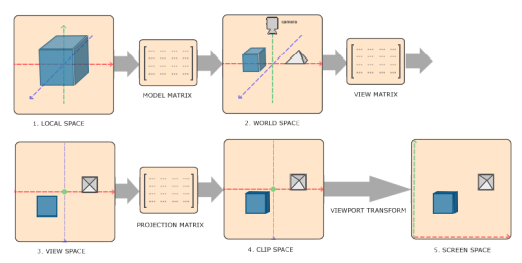
\includegraphics{space_coordinates_process.png}

Como se ve, la mayor parte de las transformaciones están hechas con matrices.
Específicamente hay tres: la \emph{matriz de modelado}, la \emph{matriz de visión} y la \emph{matriz de proyección}.

La \emph{matriz de modelado} puede traducir, escalar o rotar al objeto para moverlo de su localización inicial, modificar su tamaño o cambiar su orientación. Es decir, convierte las coordenadas locales a globales.

La \emph{matriz de visión} es la que se encarga de transformar los objetos a través de traducciones y rotaciones para traducir/rotar la escena para que se vean frente a la cámara. Estas transformaciones se le hacen a las coordenadas obtenidas en el espacio global.

Y la \emph{matriz de proyección} permite que se utilicen rangos de coordenadas como $[-3000, 3000]$ en cada eje y se le pasen así a la shader de vértices para luego normalizarlas a un rango $[-1.0, 1.0]$ que acepta OpenGL. Así todos los vértices que tengan una coordenada menor a -1.0 o mayor a 1.0 son recortados. Se ve que la matríz de proyección crea una "caja de visualización" a la que se llama \emph{frustum} en inglés, las coordenas que queden dentro del \emph{frustum} se verán en pantalla. Además, esta matriz puede ser una matriz de proyección \emph{ortográfica} o \emph{de perspectiva}.

Hay que destacar que luego de que los vértices estén en el espacio de recorte, se lleva a cabo la \emph{división de perspectiva} en la que se convierten el espacio de recorte 4D a NDC 3D. Esto se hace dividiendo las componentes $x, y, z$ entre la componente $w$.

Por último, se da la transformación de ventana gráfica (viewport), etapa en la que se mapean las NDC a los valores específicados por \lstinline{glViewport}.

\subsection{Proyección ortográfica.}
En esta se define un frustum cúbico que define el espacio de recortado donde cualquier vértice fuera de esta caja no se muestra. Se ve así:

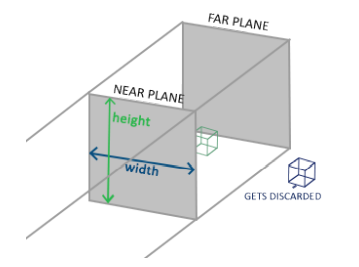
\includegraphics{ortographic_proy.png}

Lo que esté fuera del ancho, largo o esté más allá del plano lejano se recortará. Este método mapea las coordeanadas dentro del frustum a NDC sin efectos secundarios (por ejemplo, no toma en cuenta la perspectiva por lo que se pueden obtener resultados extraños) ya que no usa la componente $w$; si esta última es 0 la división de perspectiva no tiene efecto. Así se crea una matriz de proyección ortográfica con GLM:

\begin{lstlisting}
    glm::ortho(x1, x2, y1, y2, z1, z2);
\end{lstlisting}

Donde el rango x1 a x2 es el ancho, el de y1 a y2 el alto y el de z1 a z2 la distancia entre el plano cercano y el lejano.

\subsection{Proyección de perspectiva.}
Esta proyección hace que lo que esté más cerca del observador se vea más grande que lo que está lejos. La matrix de proyección de perspectiva mapea un rango de frustum dado al espacio de recortado (donde todas las coordenadas están entre -1.0 y 1.0) y manipula la componente $w$ para que se haga más grande entre más lejos el vértice. Luego de que se esté en el espacio de recorte, se hace la divisón de perspectiva en las coordenadas así:

\begin{center}
\begin{equation*}
out = \left(\begin{array}{c}
      x/w \\
      y/w \\
      z/w \\
      \end{array}\right)
\end{equation*}
\end{center}

Para crear una matriz de proyección de perspectiva en GLM se hace así:

\begin{lstlisting}
    glm::mat4 proj = glm::perspective(fov, 
                                     relacion de aspecto, 
                                     z1, z2);
\end{lstlisting}

Donde \lstinline{fov} está en radianes con \lstinline{glm::radians(grados)}, \lstinline{relacion de aspecto} es $anchura / altura$ (ambos parámetros 
de la ventana gráfica) y z1 y z2 la distancia hasta 
el plano cercano (usualmente 0.1) y hasta el plano lejano respectivamente.

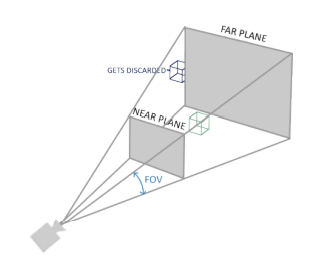
\includegraphics{perspective_proy.png}

\section{Conversión final.}
Una coordinada de vértice se convierte a una coordenada de recorte así:
\begin{equation*}
    V_{recorte} = M_{proyeccion} \cdot M_{vision} \cdot M_{modelado} \cdot V_{local}
\end{equation*}

Hay que recordar que la multiplicación de matrices se debe leer de izquierda a derecha, es decir, primero se aplica la de modelado, luego la de visión y luego la de proyección. El resultado de esto debe asignarse a \lstinline{gl_Position}.

\end{document}